\documentclass[tikz, border=4pt]{standalone}
\usepackage{tikz}
\usepackage{pgf-umlcd}
\begin{document}
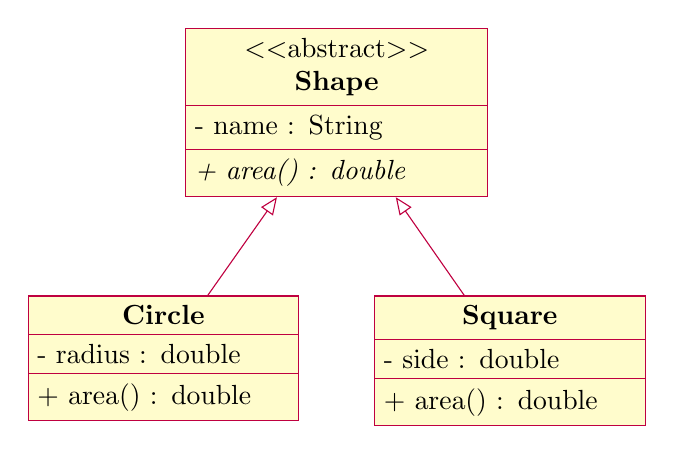
\begin{tikzpicture}[x=1cm, y=1cm]
  \begin{scope}[shift={(3.92,0)}]
    \begin{abstractclass}[text width=3.6cm]{Shape}{0,0}
      \attribute{- name : String}
      \operation[0]{+ area() : double}
    \end{abstractclass}
    \begin{class}[text width=3.2cm]{Circle}{-2.2,-3.4}
      \inherit{Shape}
      \attribute{- radius : double}
      \operation{+ area() : double}
    \end{class}
    \begin{class}[text width=3.2cm]{Square}{2.2,-3.4}
      \inherit{Shape}
      \attribute{- side : double}
      \operation{+ area() : double}
    \end{class}
  \end{scope}
\end{tikzpicture}
\end{document}
